 \subsection{Mixtures of Gaussians}

Mixtures of Gaussian is method of clustering data that's more complex than K-Means but is more effective and is able to disentangle ambiguous samples by considering probabilistic classification, known as soft assignments. 

Each cluster is modelled by a Gaussian that gives the probability density of a certain values (a sample) belong to that class. The Gaussian is initially developed by taking a histogram of all values. For one dimnesional data it would appear as in Figure \ref{fig:histGauss}. A histogram can be created for any N-dimensional data set but it becomes increasingly problematic to visualize with each additional dimension.

\begin{figure}[H]
	\centering
	\begin{subfigure}[b]{0.5\linewidth}
            \centering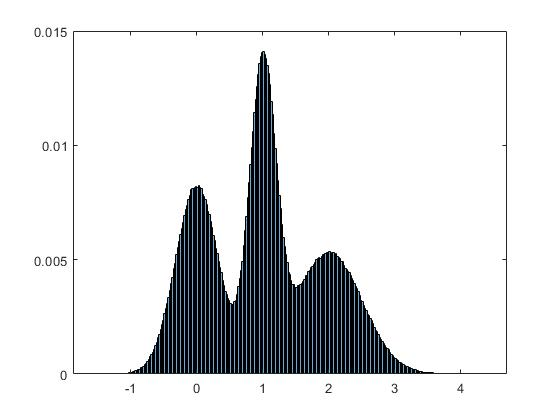
\includegraphics[width=215pt]{histGauss}
      		\caption{Normalized Histogram of 1D random samples.}
		\label{fig:histGauss}
    	\end{subfigure}%
    	\begin{subfigure}[b]{0.5\linewidth}
      		\centering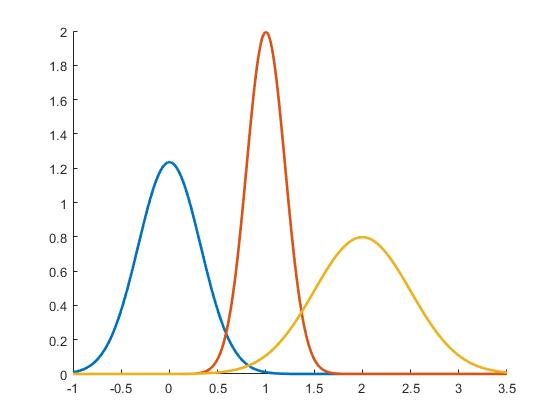
\includegraphics[width=215pt]{hist_gauss_curve}
      		\caption{Individual Gaussians derived from 1D histogram. }
       		\label{fig:histCurve}
    	\end{subfigure}
    	\caption{Formulation of Mixture of Gaussians.}
    	\label{fig:mixture}
\end{figure}

The point of interest present in the data histogram is the domain value of the 



\begin{figure}[H]
    \centering
    \centering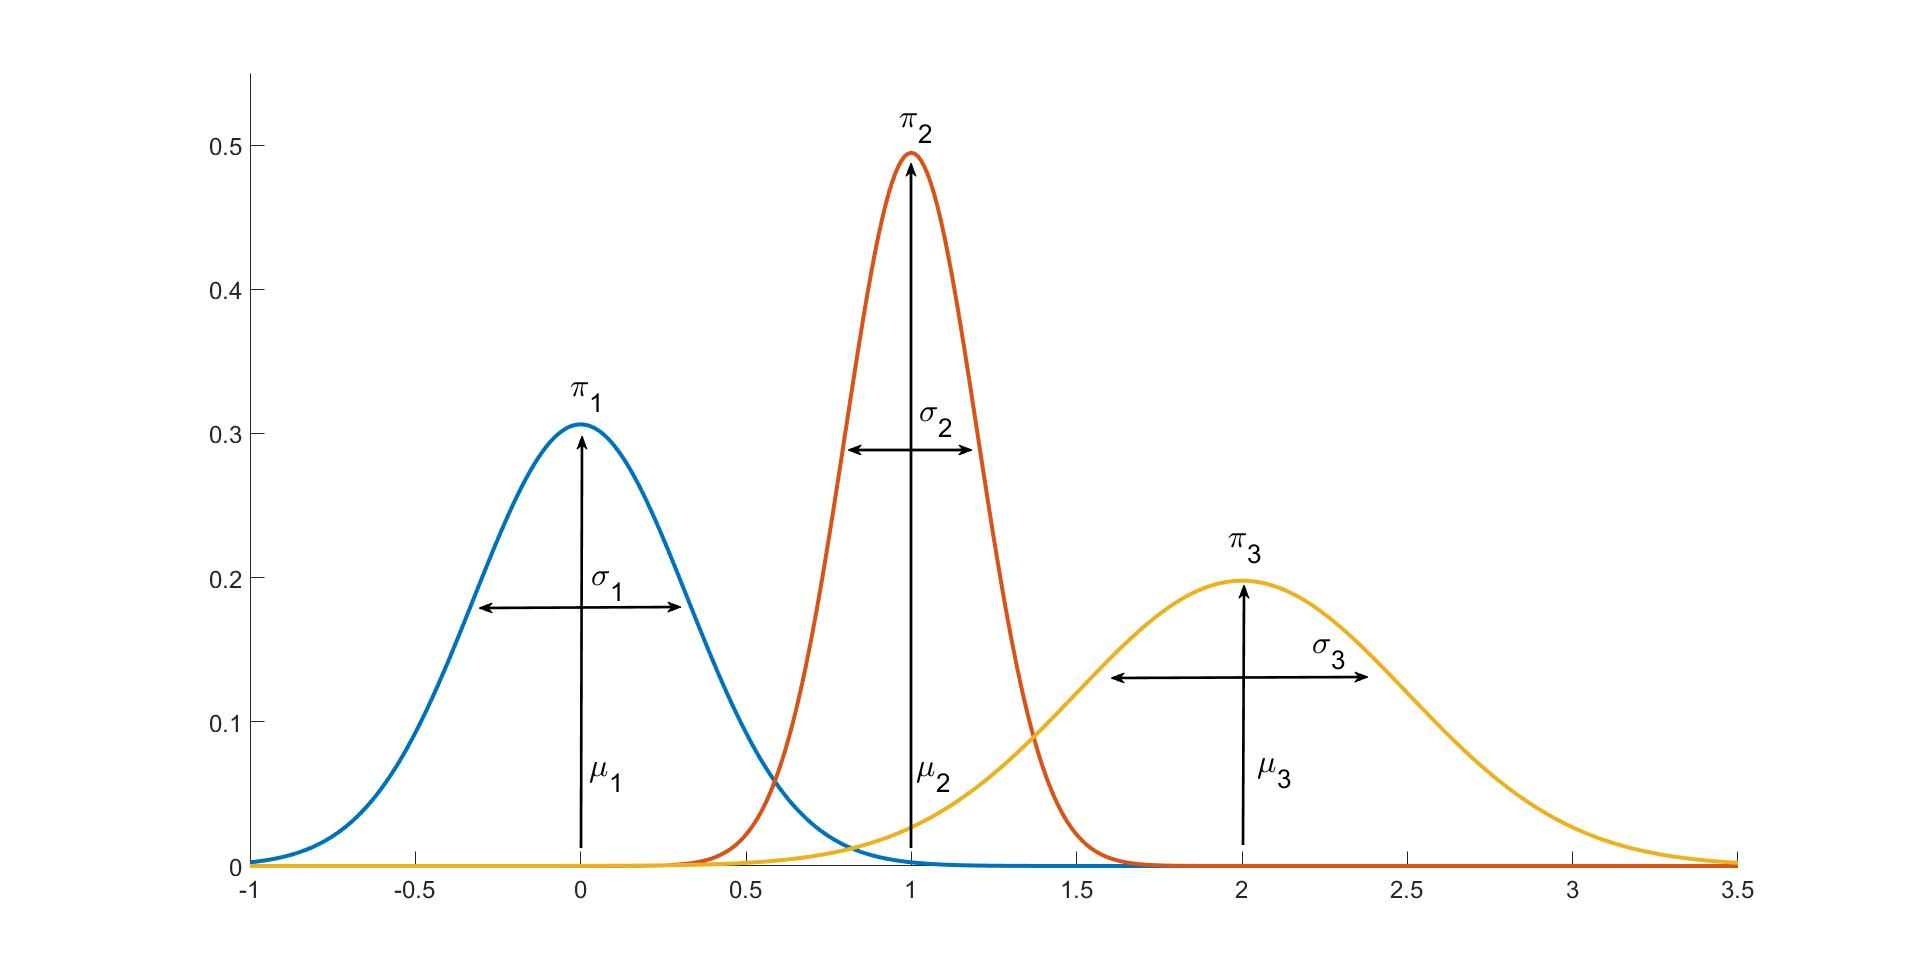
\includegraphics[width=450pt]{gauss_mix_scale}
    \caption{Individual Gaussians with scaled weightings.}
    \label{fig:histScale}
  \end{figure} 

This method is perhaps explained with an example. 




\subsubsection{Expectation Maximization}






\subsection{Background Subtraction}

This is performed by identifying a background image and then subtracting this image from subsequent frames of video to determine what has changed and hence what is a foreground image.

\subsection{Expectation Maximization}

This is an optimization scheme used to fit a Gaussian Mixture Model. It is an iterative method that faurantees convergence to a local maximum in a search space.